\documentclass[12pt,a4paper]{article}

%%% REPORT FOR SPIN WAVES EXCITATION BY ACOUSTIC PULSE

\usepackage{amsmath}               %AMSMath tools for flexible equations
\usepackage[english]{babel}
\usepackage{graphicx}
\usepackage{cite}
\usepackage[margin=1.5cm]{geometry}
\usepackage{subfig} % remplace subfigure
%\usepackage[utf8x]{inputenc} 
\usepackage[latin1]{inputenc} 
\usepackage[T1]{fontenc} 
\usepackage[section]{placeins}
\usepackage{listings} % in order to include code in a tex file
\usepackage{setspace}
\usepackage{hyperref}
\onehalfspacing

%\renewcommand{\thefootnote}{\fnsymbol{footnote}}
\renewcommand{\thefootnote}{\arabic{footnote}}
\DeclareTextSymbol{\degre}{T1}{6}

\newcommand{\valentin}{\textsc{Valentin} }
\newcommand{\vladimir}{\textsc{Vladimir} }
\newcommand{\anton}{\textsc{Anton} }
\newcommand{\alexandr}{\textsc{Alexandr} }
\newcommand{\vasily}{\textsc{Vasily} }

	
\begin{document}
	
	
\begin{center}
	{\bf\Large Meeting Recap~\MakeUppercase{\romannumeral 14}}\\
	{\bf\Large \today}\\
	\vspace{0.4cm}
	{\large Valentin \textsc{Besse}\footnote{Author of the report}, Vladimir \textsc{Vlasov}, Anton \textsc{Golov}, Alexandr \textsc{Alekhin}, Leonid \textsc{Kotov} and Vasily \textsc{Temnov}}\\
	\vspace{0.6cm}
	%{\large \today}
	%{\large August 28, 2017}
\end{center}
\vspace{0.1cm}

\section*{Version}

\begin{itemize}
    \item November 8, 2017: V1.
\end{itemize}

\section*{Present at the meeting}

\begin{itemize}
    \item Valentin \textsc{Besse}.
    \item Vladimir \textsc{Vlasov}.
    \item Anton \textsc{Golov}.
\end{itemize}

\section*{Progress}

\begin{table}[ht]
    \centering
    \begin{tabular}{|l|l|}
    \hline
    Tasks & Status \\
    \hline
    \hline
    Figures/Tables & Figures are almost done. We use figures from Rome's presentation. \\
    \hline
    Summary statements & To be done\\
    \hline
    Scientific audience & We target PRL\\
    \hline
    Materials and methods & To be done\\
    \hline
    Re-evalutate data & To be done\\
    \hline
    Results & To be done\\
    \hline
    Discussion/Conclusion & To be done\\
    \hline
    References & To be done\\
    \hline
    Introduction & To be done\\
    \hline
    Title & Acousto-magnonic cavity with exchange magnon in the THz regime\\
    \hline
    Conclusion paragraph & To be done \\
    \hline
    \end{tabular}
    \caption{Sum up of the tasks and the progress. The tasks' division follows the algorithm describe in Fig. 1 of \cite{o2009algorithm}}
    \label{tab:my_label}
\end{table}

\section*{Agenda}

During this meeting we discuss about:
\begin{enumerate}
    \item progress on the paper.
    \item results with anisotropy.
    \item questions.
\end{enumerate}

The pad used during the meeting can be found \href{https://pad.aumbox.net/mypads/?/mypads/group/exchange-magnons-4m3cvuz/pad/view/2017-11-08-meetingsyktyvkar-z2b7v30}{here}\footnote{https://pad.aumbox.net/mypads/?/mypads/group/exchange-magnons-4m3cvuz/pad/view/2017-11-08-meetingsyktyvkar-z2b7v30}.

\section{Progress on the paper}

\valentin uploaded 2 new figures.
He will add two figures:
\begin{itemize}
    \item a spectrum for different damping.
    \item a sketch for the experiment.
\end{itemize}
After that He will start to work on the theory part.
It seems reasonable to think that a part of the theory part will be in the supplementary material.
After that he will write on the descriptions of the results.

\section{Results with anisotropy}

\vladimir worked on the anisotropy in nickel films.
He found two type of anisotropy: cubic and uniaxial.

\anton presented his study about the impact of the anisotropy.
It changed the excitation of the mode
\begin{figure}
    \centering
    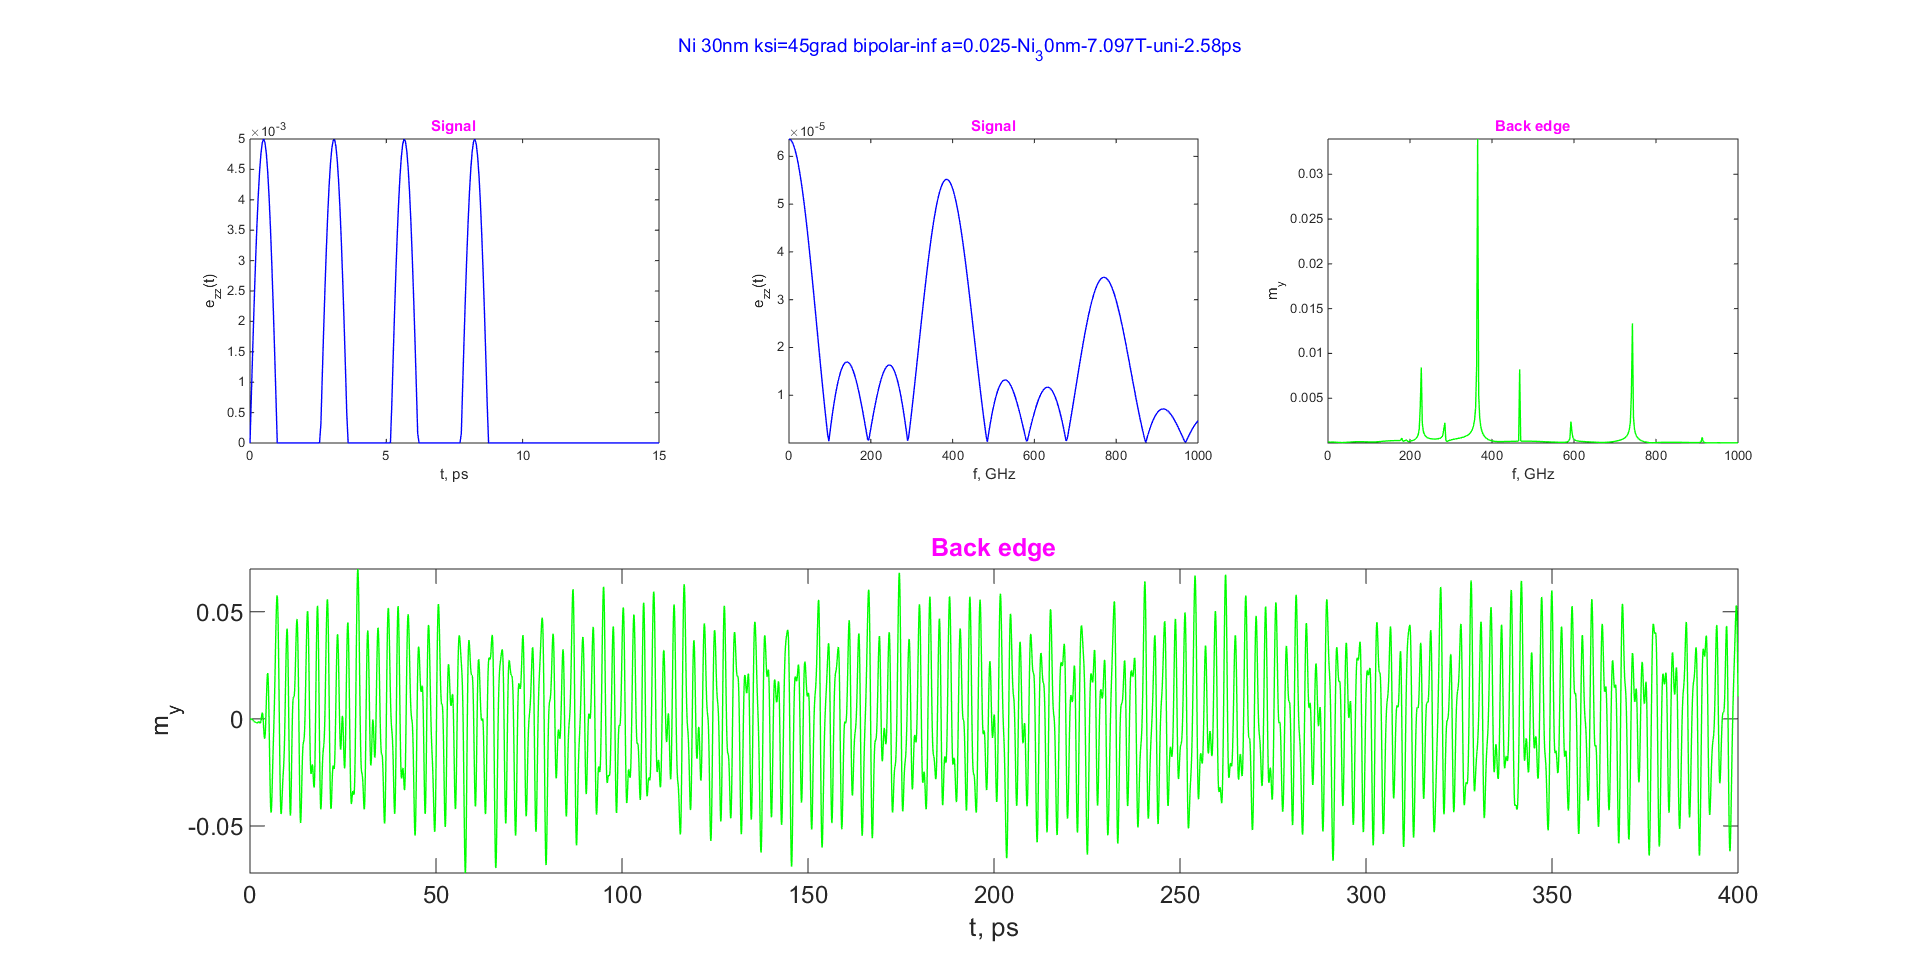
\includegraphics[width=0.95\textwidth]{cubic.png}
    \caption{Ni film (30nm) with $H = 7_097\ \mathrm{T}$ exited by 4 unipolar acoustic pulses separated by $2. 58\ \mathrm{ps}$ without Gilbert damping. It is the case with the cubic anisotropy.}
    \label{fig:cubic}
\end{figure}
\begin{figure}
    \centering
    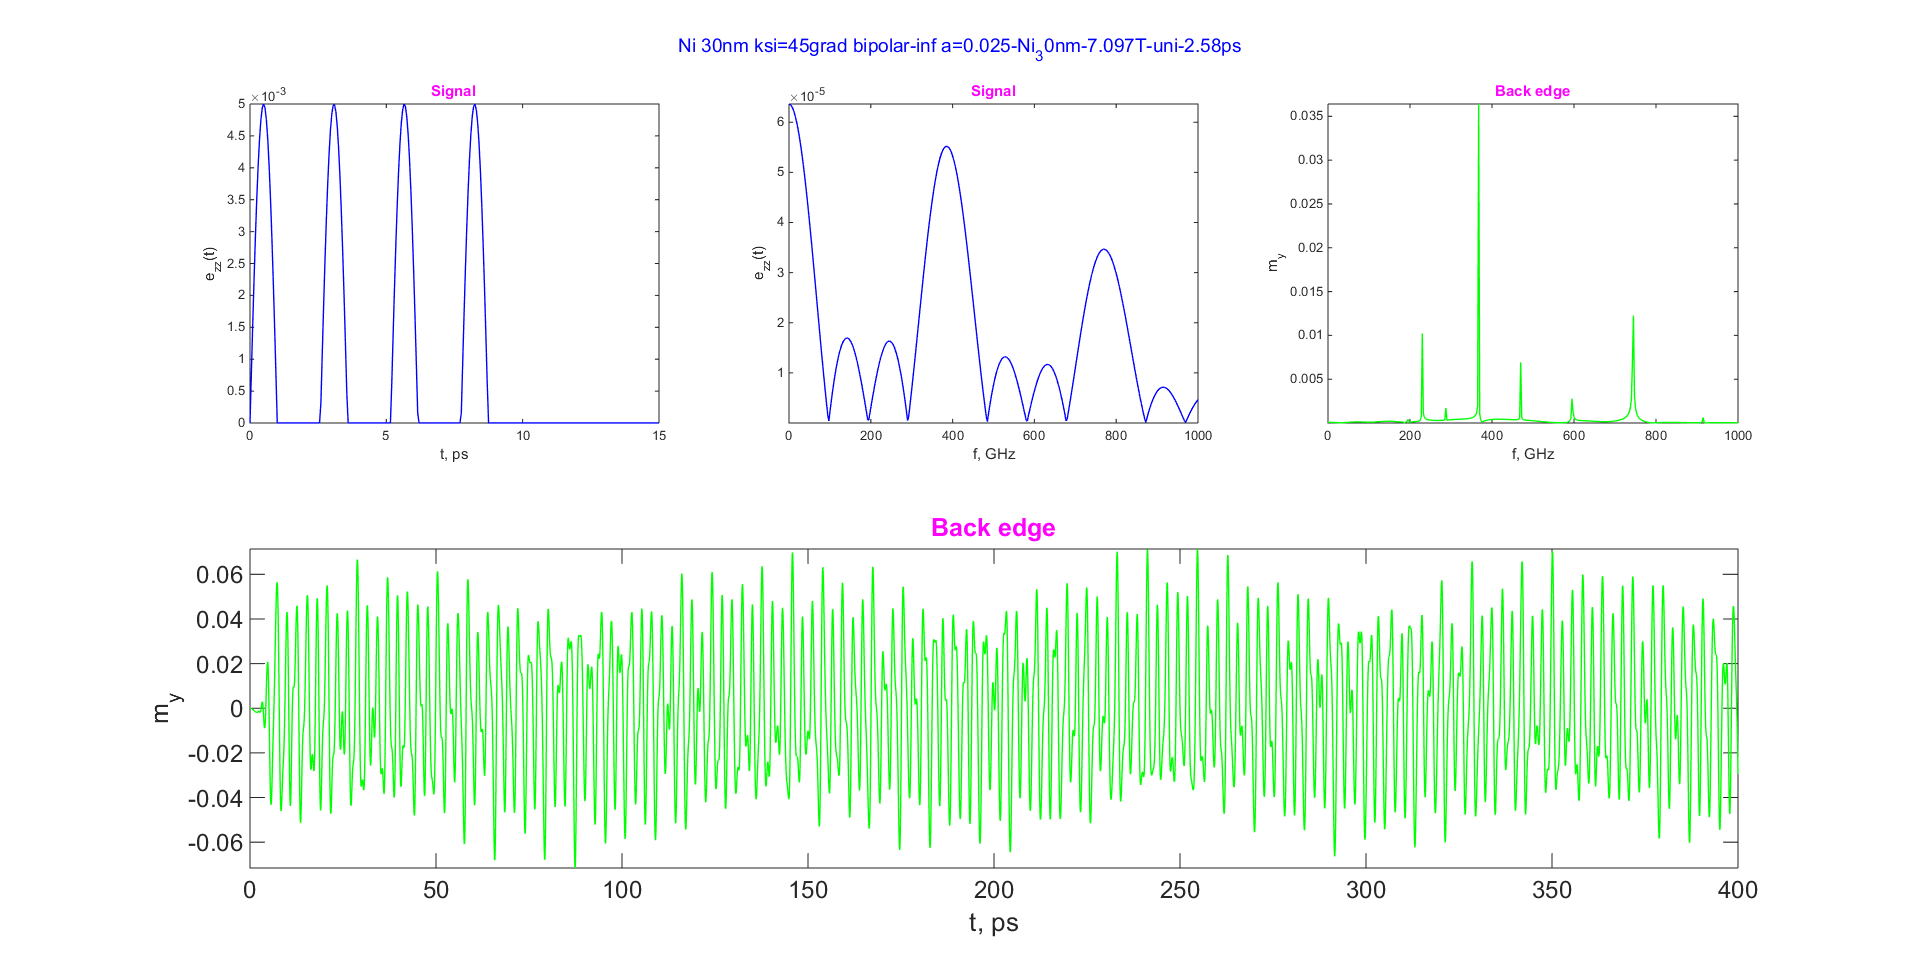
\includegraphics[width=0.95\textwidth]{uniaxial.png}
    \caption{Ni film (30nm) with $H = 7_097\ \mathrm{T}$ exited by 4 unipolar acoustic pulses separated by $2. 58\ \mathrm{ps}$ without Gilbert damping. It is the case with the uniaxial anisotropy.}
    \label{fig:uniaxial}
\end{figure}
\begin{figure}
    \centering
    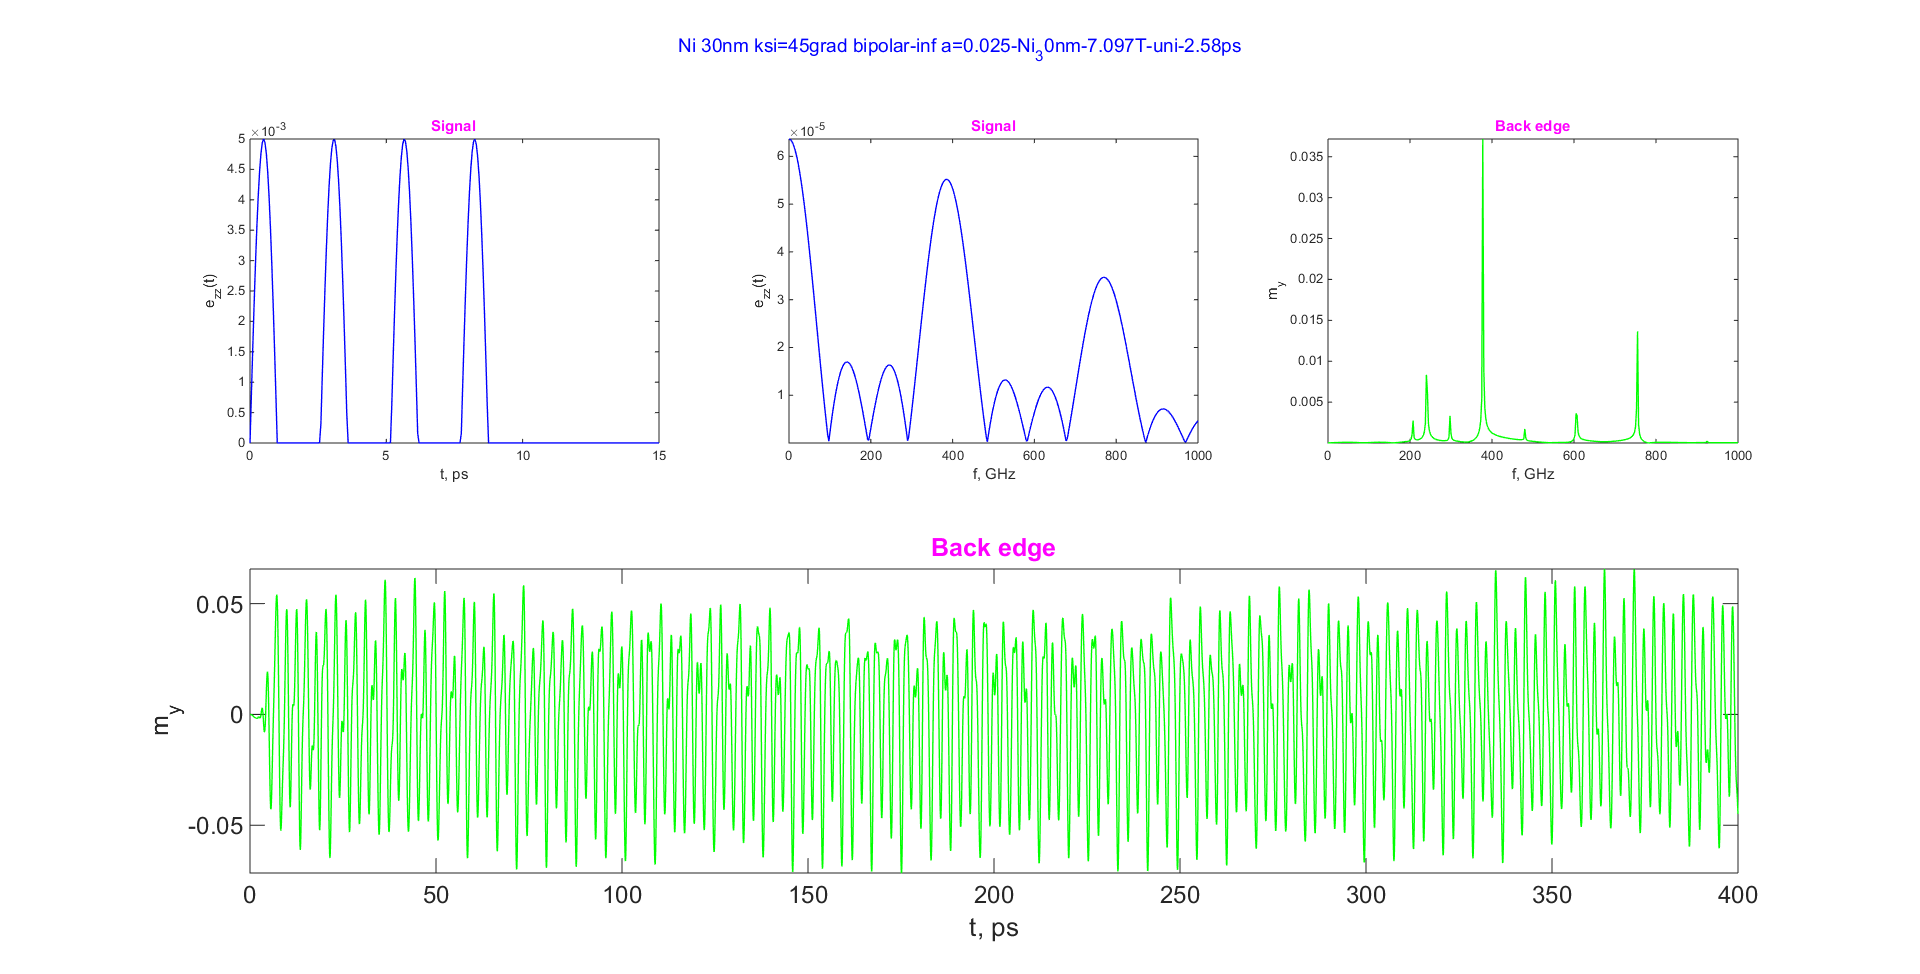
\includegraphics[width=0.95\textwidth]{none.png}
    \caption{Ni film (30nm) with $H = 7_097\ \mathrm{T}$ exited by 4 unipolar acoustic pulses separeted by $2. 58\ \mathrm{ps}$ without Gilbert damping. There is no anisotropy.}
    \label{fig:none}
\end{figure}

We should plot the divergence of the dispersion relation for the different anisotropy types.

\section{Questions}

Alexandr asks:
\begin{itemize}
    \item could we give realistic units for the precession angle ? Valentin wants to know about the unit of $m_x$, $m_y$ and $m_z$.
    \item we should compare the amplitude of the acoustic pulses and the amplitude of the precession (in realistic units).
    \item we should compare the value of the constant of the phonon-magnon interactions ($b_1$) with the electron-phonon interactions.
\end{itemize}

Answers:
\begin{itemize}
    \item yes, it is possible to give measurement of the precession angle. The value of $\vec{m}$ (unit magnetization vector) corresponds to the position (x-, y- and z-axis). 
    \item we can measure the amplitude of the precession (in realistic units) by fitting the temporal trace using the definition of the magnetization vector.
    \item In Ni, the electron-phonon interaction is higher than Co and Fe. We should give number from paper.
\end{itemize}

Valentin asks:
\begin{itemize}
    \item $b_1$ is in $\mathrm{J}/\mathrm{m}^3$ (energy density).
    \item from discussion with Vasily. Also Leonid Kotov think that the magnetoelastic effect is frequency depedant.
    \item $\partial \vec{m} / \partial t = 0$ at $z = 0,\ L$.
\end{itemize}

\section*{Next meeting}

The next meeting will be Monday November 13th at 2:00 pm (CET).

\newpage

\section*{List of abbreviations}

\begin{table}[ht]
    %\centering
    \begin{tabular}{ l c r }
        Landau-Lifschitz-Gilbert & $\Longrightarrow$ & LLG \\
        Ferromagnetic resonance & $\Longrightarrow$ & FMR \\
    \end{tabular}
\end{table}

\bibliographystyle{ieeetr}
\bibliography{Exchange_Magnons}

\end{document}